\section{Architecture}
In the following, we describe the architecture of helios, which is currently designed as shown in Figure ~\ref{fig:hardarchitecture}: helios acts as an intermediary layer between the game as a real-time data model~\cite[525]{Gre19} and the technical infrastructure.
The framework visualizes the game state and transmits input data to the game as control commands.

\begin{figure}[!h]
    \centering
    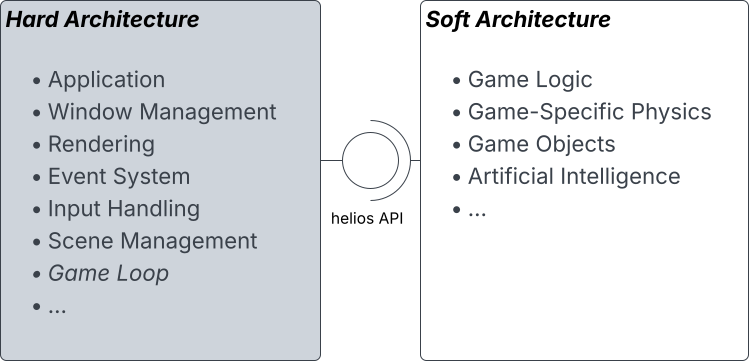
\includegraphics[width=1\columnwidth]{img/hardarchitecture_en.svg}
    \caption{Division of the architecture of the helios framework into \textit{hard} and \textit{soft architecture} according to Rollings and Morris~\cite[612 ff.]{RM04}. The ball/socket notation illustrates that helios provides interfaces that can be used by any game. (Source: own representation)}

    \label{fig:hardarchitecture}
\end{figure}

Figure~\ref{fig:package_diagram} shows a more detailed view of the modules and selected components.
The directory structure of helios reflects the structure of its core functionalities.
In the sense of \textit{Evans}, this is crucial for high cohesion: The directory names communicate the functionalities they contain~\cite[180 f.]{Eva03}.
Within the modules, there is a further subdivision into layers (such as \texttt{controller}), which is referred to as ``package-by-feature and -by-layer``.


\begin{figure*}[t]
    \centering
    \makebox[\textwidth][c]{% Box is text-width, content may extend beyond
        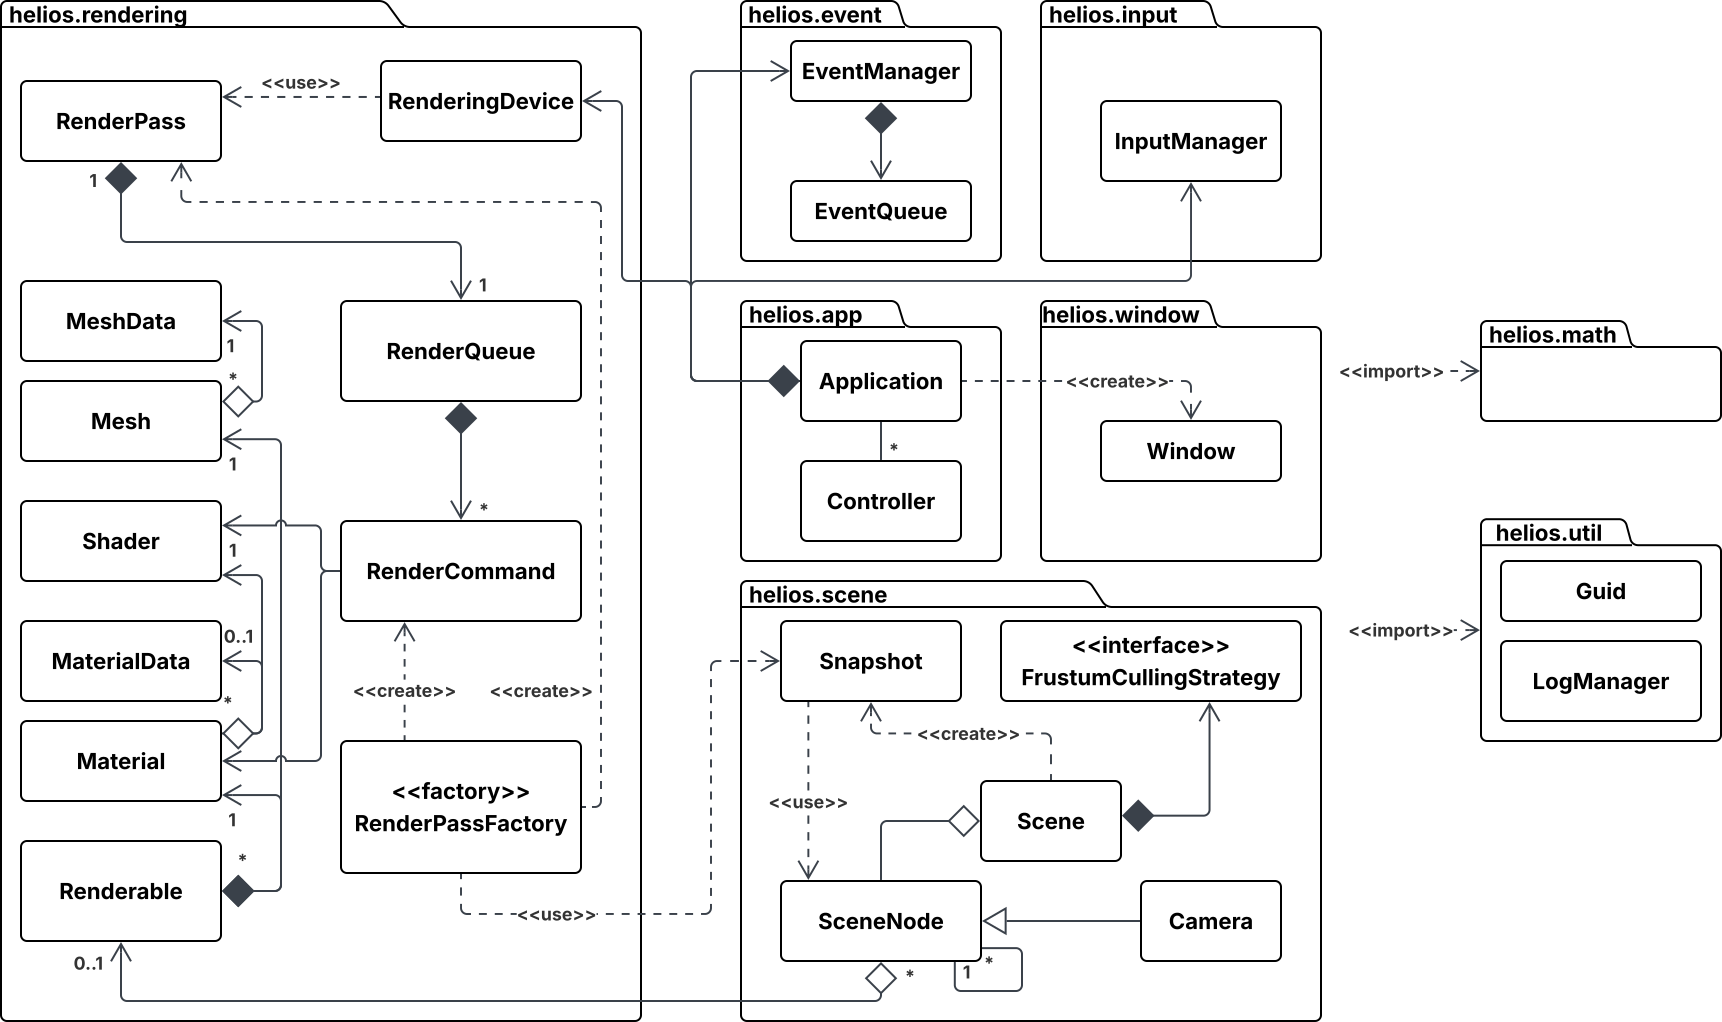
\includegraphics[width=1\textwidth]{img/package_diagram.svg}% \linewidth == column width
    }
    \caption{Structure of the helios framework and relationship between some selected components. The modules are structured according to a ``by-feature, by-layer`` concept, in which features are divided internally into functional layers. (Source: own representation)}

    \label{fig:package_diagram}

\end{figure*}


\subsection*{\texttt{app}: Application layer}
The central control unit of the application or game is the \texttt{Application} class, which provides the event system, input processing, and window management, and initializes the rendering backend - represented by \texttt{RenderDevice}.
helios also supports dynamic addition of application controllers~\cite[379] {Fow03} for defining isolated, event-based control logic, such as behavior during a window resize\footnote{
    The application controllers were originally introduced to abstract ``framebuffer resize`` events from the rendering backend.
}.

\subsection*{\texttt{input}: Input processing}
The \texttt{InputManager} orchestrates input processing.
It is managed exclusively by the application and bound to the active window.
A specialized \texttt{InputAdapter} abstracts the input events provided by the TPLs and translates them for the \texttt{InputManager}.
At the beginning of the game loop, active input events are polled (\texttt{InputManager::poll()}). Events are queried using methods such as \texttt{InputManager::isKeyPressed()}.

\subsection*{\texttt{event}: Event processing}
Events can be written to an \texttt{EventQueue} (``\textit{post}``) via the \texttt{EventManager}.
Interested observers (\textit{Observer}) can register with the \texttt{EventManager} via callbacks using \texttt{subscribe}~\cite[293 ff.]{GHJV94}.
The method \texttt{EventManager::dispatchAll()} informs the observers about existing events.

\subsection*{\texttt{window}: Window class}
The \texttt{Window} class provides interfaces for controlling the application window, querying window events, and instructing \textit{buffer swapping}.


\subsection*{\texttt{math}: Mathematical types and operations}
This module provides trigonometric functions and representatives for data types anchored in linear algebra, such as vectors and matrices, in the namespace \texttt{helios::math}.
It also supports operations for linear and affine transformations, thereby implementing the coordinate space change commonly used in 3D computer graphics\footnote{
    After projection, the coordinates are available in the so-called clip space.
    Typically, the rendering backend uses perspective division to convert these coordinates into NDC (\textit{Normalized Device Coordinates}) relevant for the rasterizer~\cite[18]{AHHP+18}.
}:

\[
    \text{Model}\rightarrow\text{World}\rightarrow\text{View}\rightarrow\text{Projection}
\]

\noindent

The interfaces are based on popular libraries such as the aforementioned \texttt{glm} for their method signatures.

\subsection*{\texttt{scene}: Scene graph}
The scene graph \texttt{helios::scene::Scene} follows established implementations from the literature\footnote{See, among others,~\cite[]{She07} and~\cite[]{Gre19}.}.
\texttt{Scene} has an implicit root node that can contain any number of child nodes.
Each \texttt{SceneNode} has a \texttt{Transform} object that describes the model transformation in the local coordinate system.
\texttt{SceneNodes} can be ``renderable``, i.e., they are configured with a \texttt{Renderable}.
However, they can also simply represent a camera (\texttt{helios::scene::Camera})\footnote{
    In this context, other node types usually include (freely positionable) \texttt{LightNodes}, i.e., light sources.
}.
Scene nodes with \texttt{Renderable} are taken into account during \textit{culling}.
The culling procedure is defined abstractly in the purely virtual class \textit{FrustumCullingStrategy}. Specializations are passed to the \texttt{Scene} during instantiation.
In the application stage~\cite[687]{Gre19}, helios creates a \texttt{Snapshot} from a scene and a camera, for which the configured culling strategy collects all \texttt{SceneNode}s located in the camera's visible area.
A single snapshot forms the basis for a \texttt{RenderPass}, which contains the necessary instructions (\texttt{RenderCommand}s) for the actual rendering process.
Listing~\ref{lst:gameloop} shows the sequence of a simple game loop.


\begin{lstlisting}[style=c++style, caption={Implementation of a simple game loop in helios. A \texttt{snapshot} is created from the scene, which serves as the basis for the \texttt{RenderPass}.}, label=lst:gameloop]
while (!win->shouldClose()) {
  app->eventManager().dispatchAll();

inputManager.poll(0.0f);

  if (inputManager.isKeyPressed(Key::ESC)) {
      win->setShouldClose(true);
  }

snapshot   = scene->createSnapshot(*camera);
renderPass = factory.buildRenderPass(
    snapshot
  );

app->renderingDevice().render(renderPass);

  win->swapBuffers();
}
\end{lstlisting}



\subsection*{\texttt{rendering}: Render Pipeline}
The rendering system of helios is divided into different modules, including \texttt{shader} for shader and GLSL\footnote{\textit{OpenGL Shading Language}}-specific code, and \texttt{model} for abstractions of material and mesh data.
\texttt{Renderable}s are representatives of ``renderable`` objects.
They encapsulate information necessary for the rendering process and are modeled as aggregations.
They consist of individually configurable \texttt{Material} and \texttt{Mesh} instances, which in turn share \texttt{MaterialData} and \texttt{MeshData} objects with other instances for easy and resource-efficient reuse~\cite[126]{AHHP+18}.

The information required for a \texttt{RenderPass} is collected as \texttt{RenderCommand} objects in a \texttt{RenderQueue}, which are processed by the actual \texttt{RenderDevice}: \texttt{RenderCommand}s have pointers to the geometry to be rendered (\texttt{Mesh}), the \texttt{Shader} to be used, and data objects in which information about \texttt{Uniform} variables (transformation matrices, etc.) is stored.
The \texttt{RenderDevice} processes a \texttt{RenderPass} using the template methods \texttt{preRender, doRender}, and \texttt{postRender}.


\subsection*{\texttt{util}: Utility classes}
The \texttt{helios::util} module contains non-domain-specific code, such as the \texttt{LogManager} for simple logging functions and a \texttt{Guid} implementation for configuring objects with a global unique identifier (\textit{global unique identifier}).